\section{Physics Performance}
\label{sec{physicsperformance}}

\subsection{Sensitivity to hidden sector particles}

\subsection{Sensitivity to LDM}
\begin{itemize}
    \item Simulation of LDM production and interaction: MadDump and FairShip (Figure \ref{fig:ldm_prod})
    
    \begin{figure}[htbp]
    \centering  
    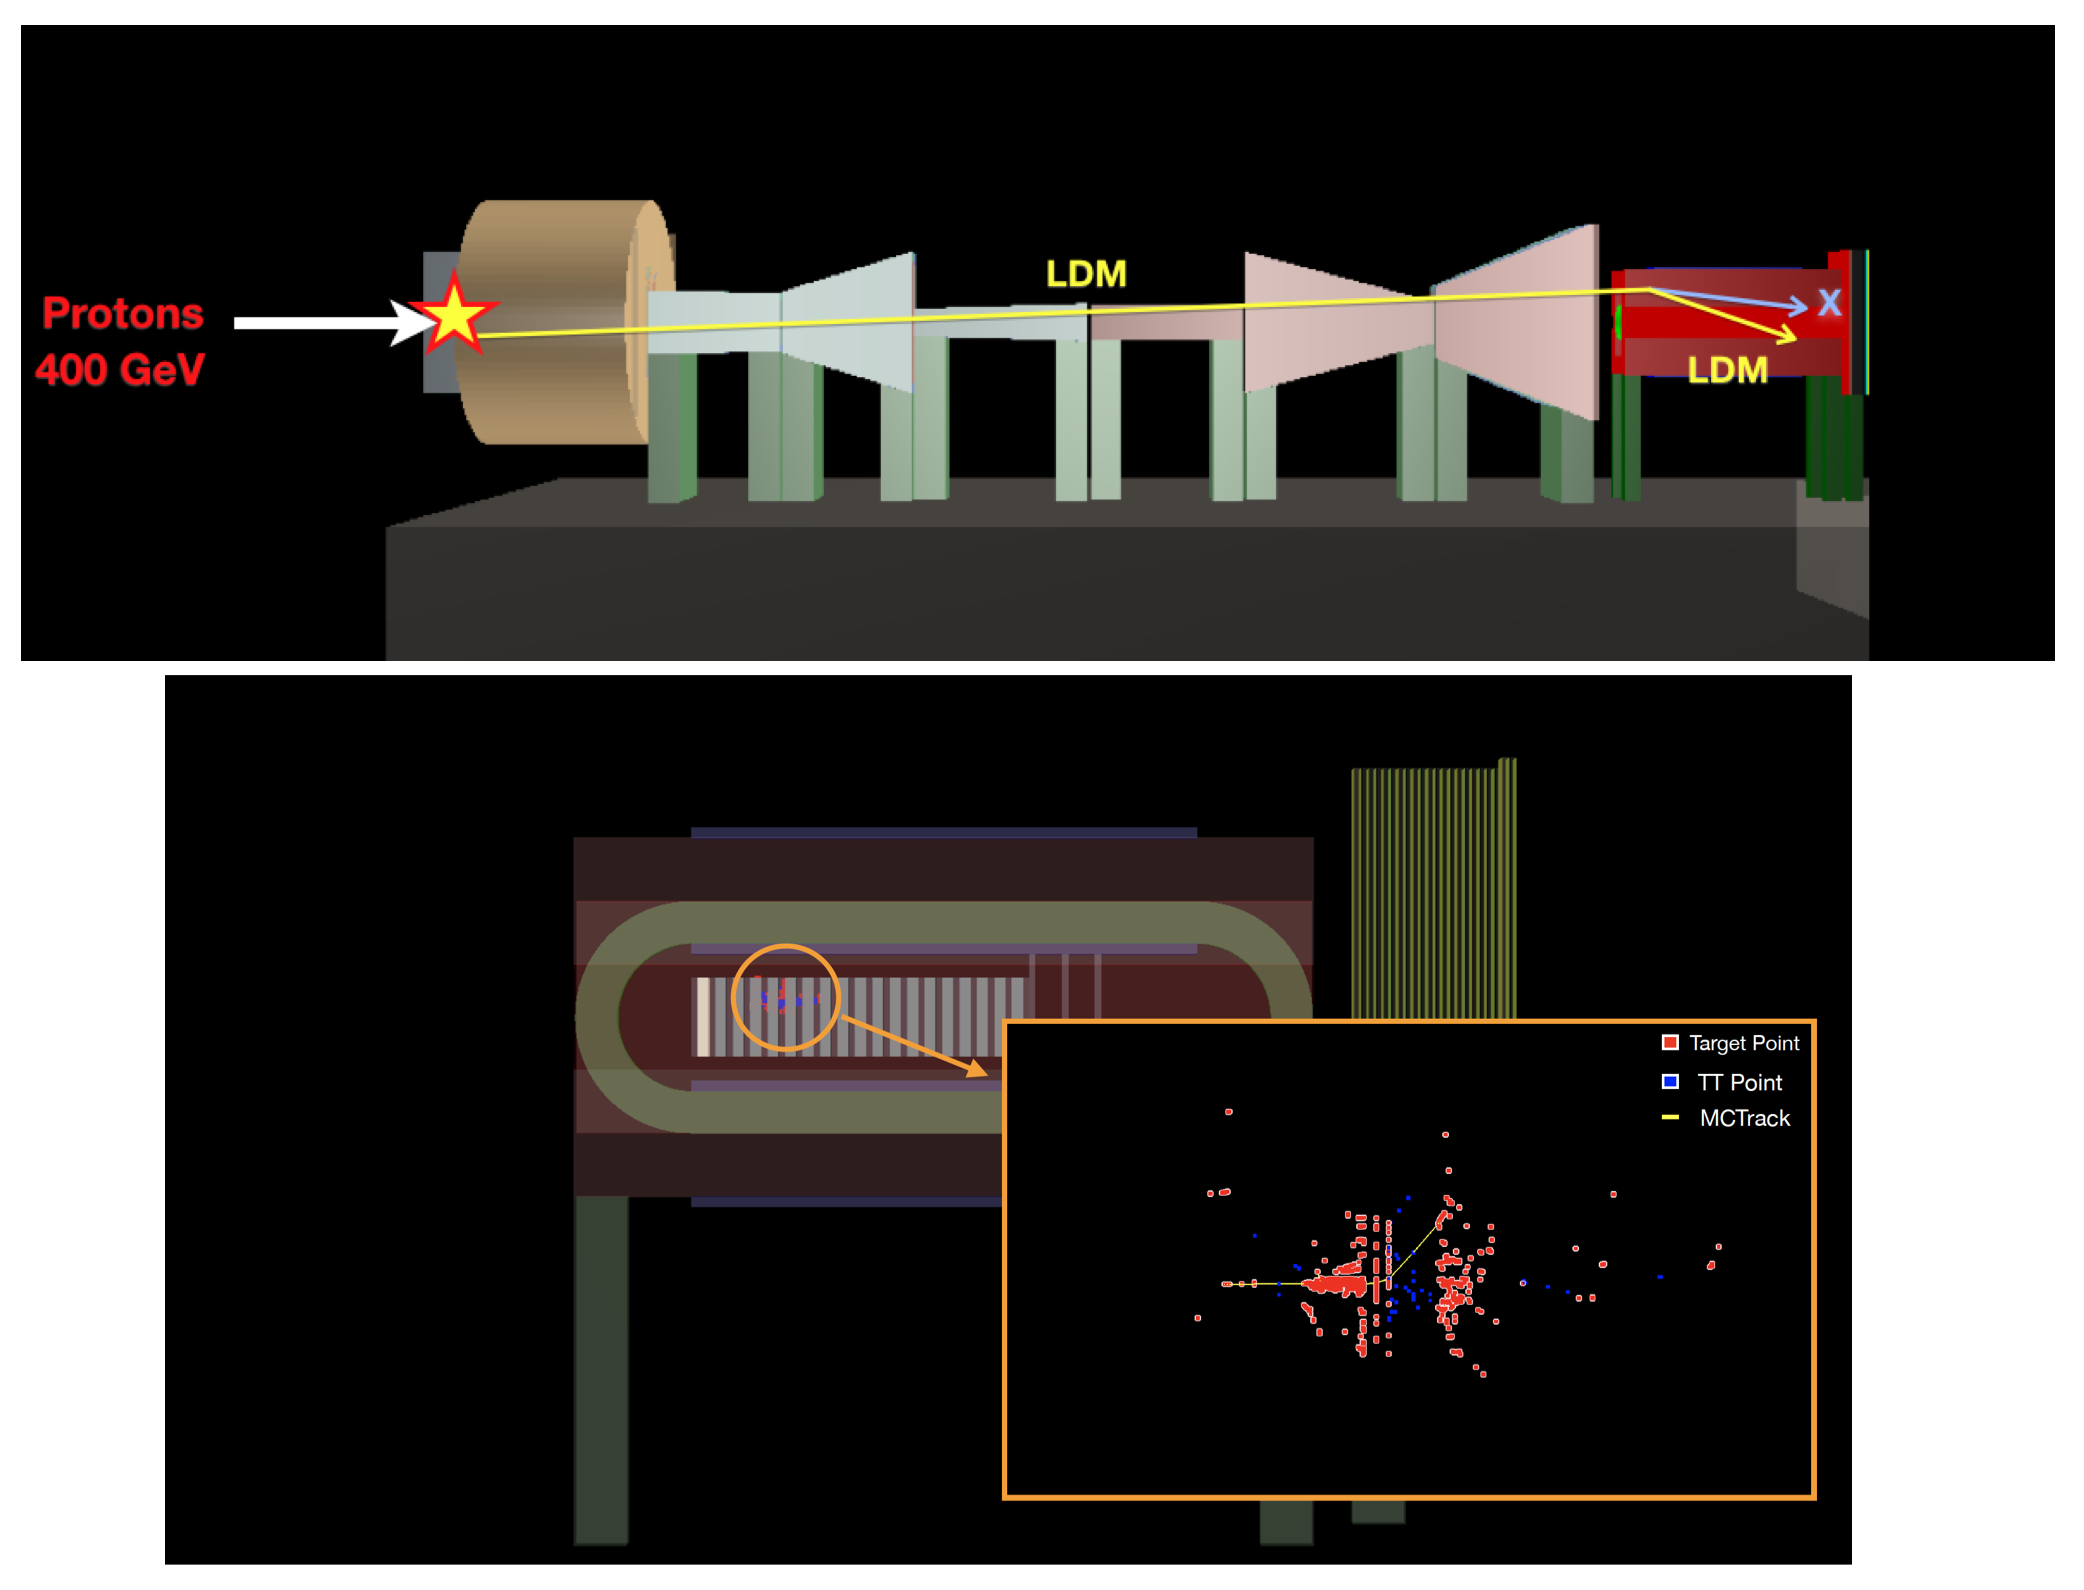
\includegraphics[scale=0.3]{figs/PhysicsPerformance/LDM_Prod.png}
    \caption{Light Dark Matter simulation process design in two steps. The first one is handled by MadDump and concerns the BSM particle production and consequent decay/interaction inside the detector; the second stage consists in the particles propagation inside the SHiP detector and is owned by FairShip.}
    \label{fig:ldm_prod}
    \end{figure}

    \item Neutrino background yield estimation
    \begin{itemize}
        \item[$\circ$] Kinematic distribution for neutrino background (Figure \ref{fig:ldm_back})
         \item[$\circ$] Selection criteria: 1 GeV $< E_e <$ 20 GeV, 10 mrad $<\theta_e<$ 20 rad
   \item[$\circ$] Neutrino background yield (Table \ref{tab:ldm_back})
    
      \begin{figure}[htbp]
    \centering  
    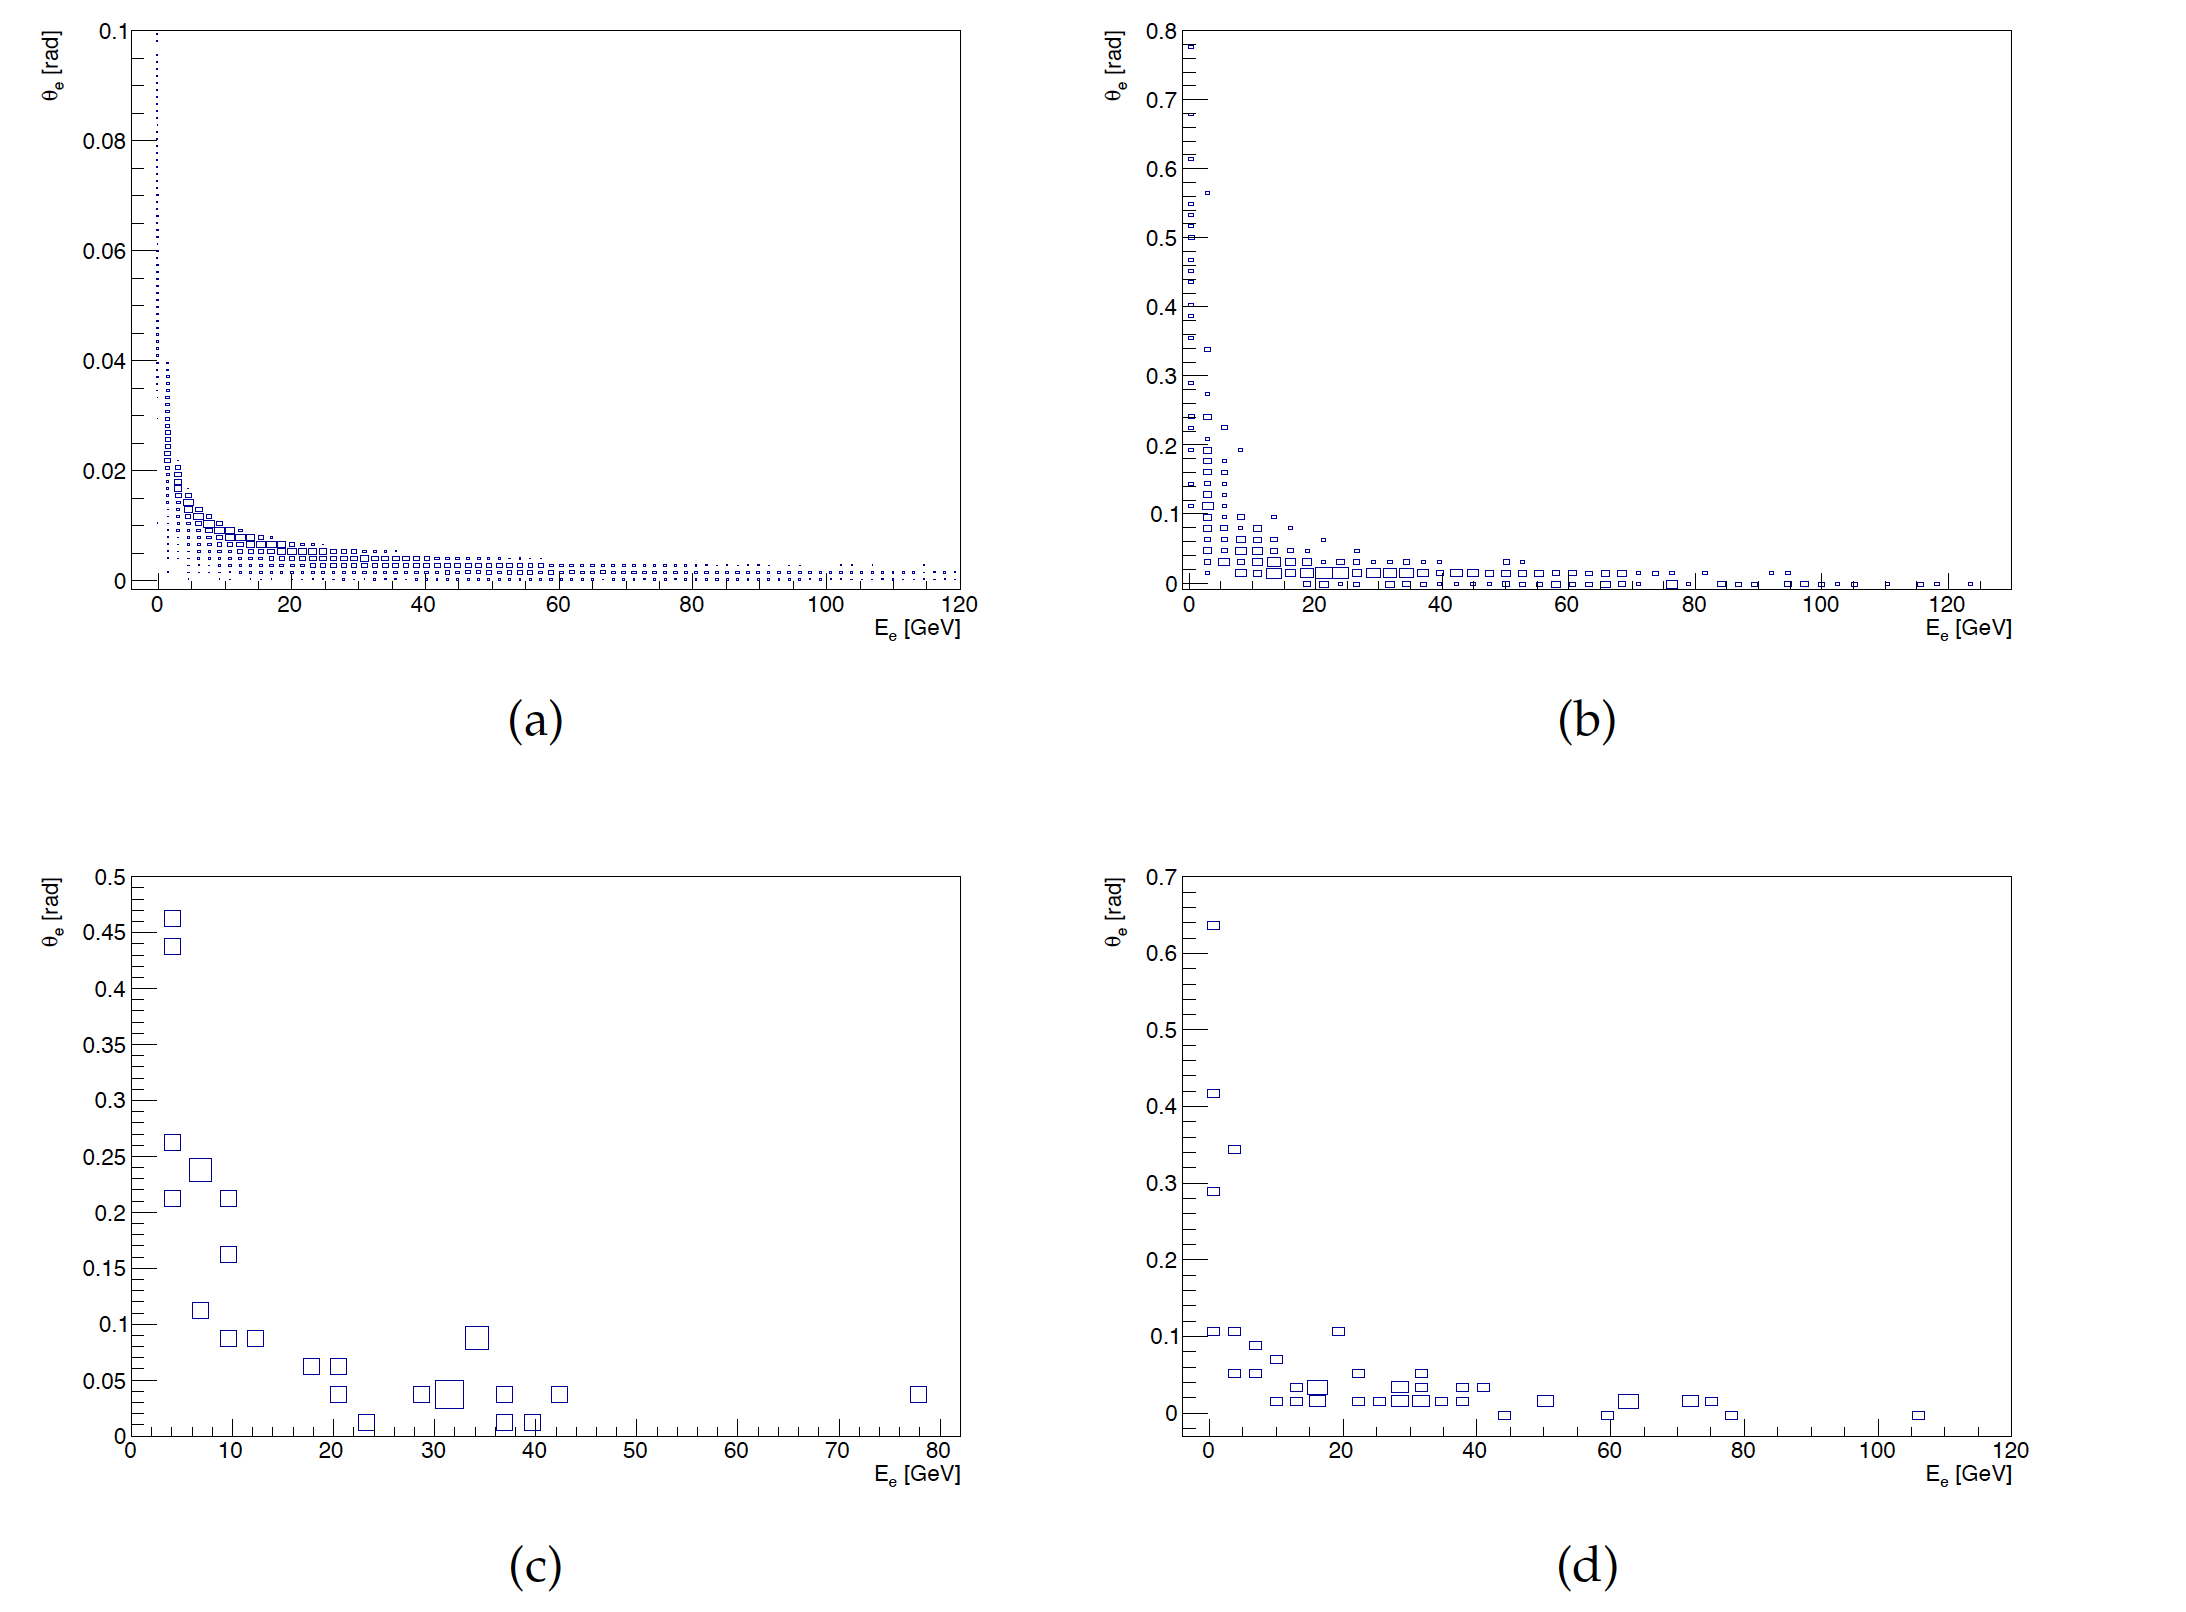
\includegraphics[scale=0.3]{figs/PhysicsPerformance/LDM_back.png}
    \caption{Electron scattering angle w.r.t. the incoming neutrino direction versus the electron energy in case of: (a) elastic, (b) quasi-elastic, (c) deep inelastic and (d) resonant scattering.}
    \label{fig:ldm_back}
    \end{figure}
    
    \begin{table}[htbp]
    \begin{center}
    \begin{tabular}{llllll}
    \hline
    & $\nu_e$ & $\bar{\nu_e}$ & $\nu_\mu$ & $\bar{\nu_\mu}$   & all  \\
    \hline
    Elastic Scattering on $e^-$   & 81  & 45  & 56 & 35 & 217\\
    Quasi-elastic Scattering      & 245 & 236 & -  & -  & 481 \\
    Resonant Scattering           & 16  & 162 & -  & -  & 178\\
    Deep Inelastic Scattering     &  -  & 14  & -  & -  & 14\\
    \hline
    total                         & 342 & 457 & 56  & 35& 890\\
 
    \end{tabular}
    \label{tab:ldm_back}
    \caption{Number of  background events for LDM search after cuts with 2$\times 10^{20}$ p.o.t.}  
    \end{center}
    \end{table}

    
     \end{itemize}
     
    \item Sensitivity to LDM
    \begin{itemize}
        \item[$\circ$] Model used for the simulation
        \item[$\circ$] Exclusion plot (Figure \ref{fig:ldm_sensitivity})
   \end{itemize}
    
     \begin{figure}[htbp]
    \centering  
    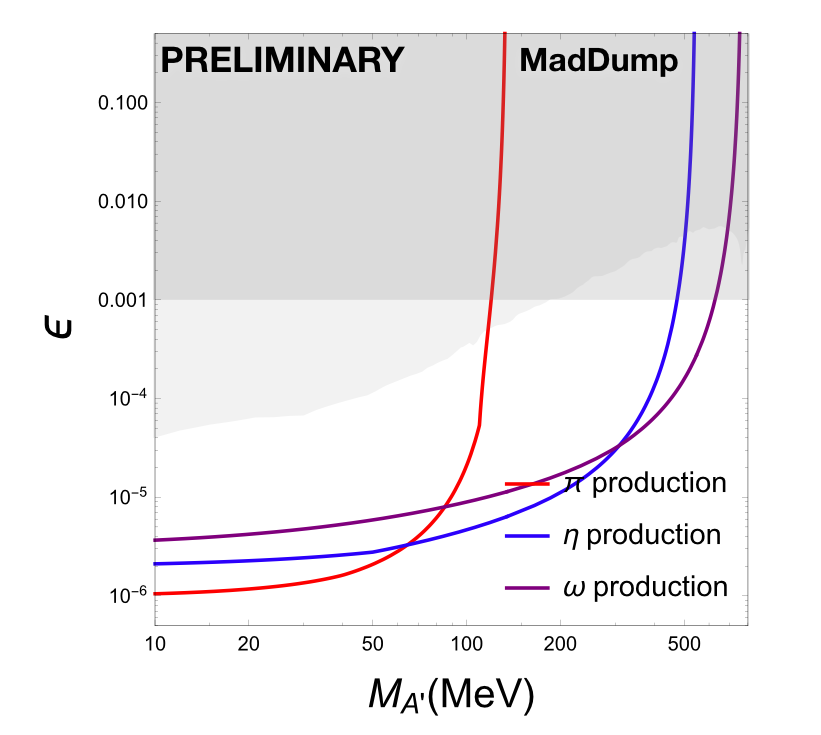
\includegraphics[scale=0.3]{figs/PhysicsPerformance/newsens.png}
    \caption{SHiP estimated sensitivity to Light Dark Matter from Dark Photon $A'$ decays in the plane ($\epsilon$, $M_{A'}$ ), in case the latter is produced in the decay of mesons. The grey shaded regions determine the parameter space which has been already ruled out by BaBar and MiniBooNE searches.}
    \label{fig:ldm_sensitivity}
    \end{figure}
    
    
\end{itemize}




\subsection{Physics with neutrinos}

\begin{itemize}
    \item Neutrino yield estimation
        \begin{itemize}
        \item[$\circ$] Energy spectra for different neutrino flavors  (Figure \ref{fig:neu_spectra})
        \item[$\circ$] Neutrino yield for different neutrino flavors  (Table \ref{tab:neu_yield})
        \item[$\circ$] Expected $\nu_\tau$ and $\overline{\nu}_\tau$ yield in different decay channels
         (Table \ref{tab:tau_yield})
        \end{itemize}

 \begin{figure}[htbp]
    \centering  
    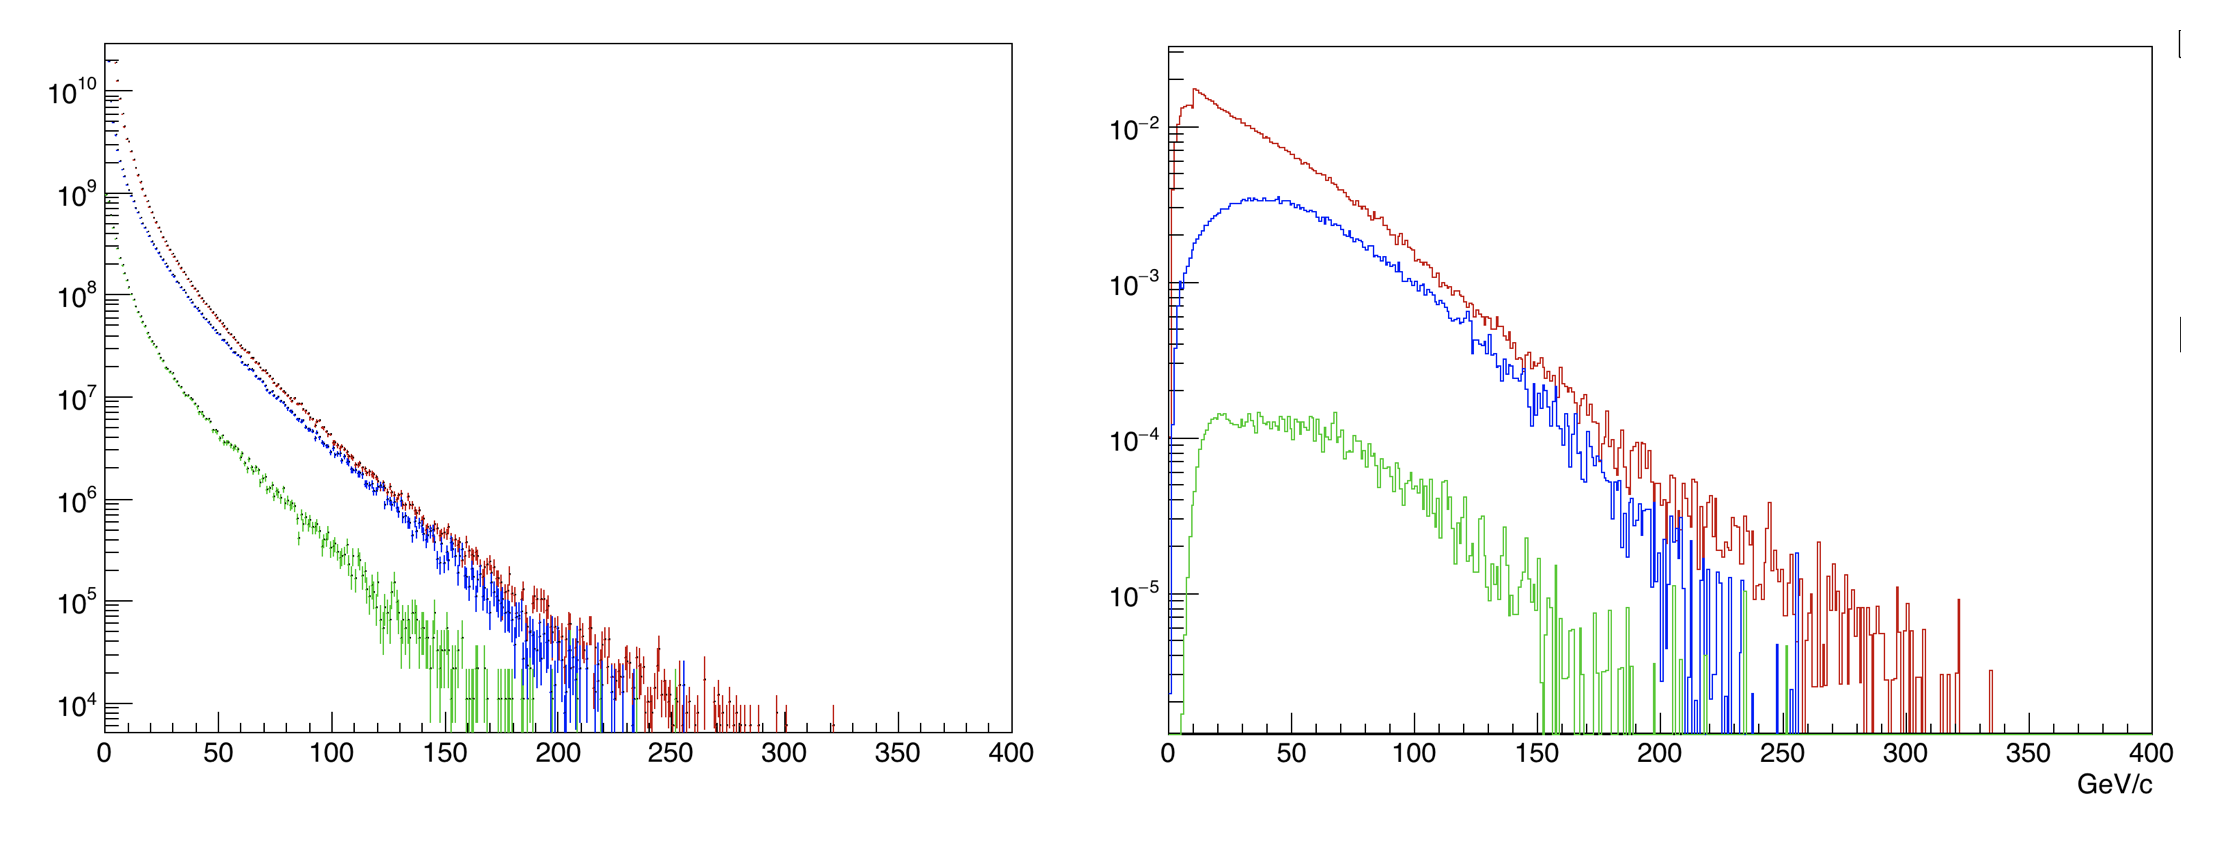
\includegraphics[scale=0.4]{figs/PhysicsPerformance/neu_spectra.png}
    \caption{Energy spectra of the different neutrino flavors  at the beam dump (left) and charged-current deep-inelastic interactions (right).}
    \label{fig:neu_spectra}
    \end{figure}
    
\begin{table}[htp]
\begin{center}
\begin{tabular}{c | c c  | c c  }
\hline
& $<$E$>$  & Beam  & $<$E$>$ &  CC DIS\\
&       (GeV) & dump  & (GeV) & interactions \\
 \hline
 $N_{\nu_e}$                 & 4.1 & $2.8 \times 10^{17}$    & 59 & $1.1 \times 10^{6}$ \\
 $N_{\nu_\mu}$               & 1.5 & $4.2 \times 10^{18}$    & 42 & $2.7 \times 10^{6}$ \\
 $N_{\nu_\tau}$              & 7.4 & $1.4 \times 10^{16}$    & 52 & $3.2 \times 10^{4}$ \\
 $N_{\overline{\nu}_e}$      & 4.7 & $2.3 \times 10^{17}$    & 46 & $2.6 \times 10^{5}$ \\
 $N_{\overline{\nu}_\mu}$    & 1.6 & $2.7 \times 10^{18}$    & 36 & $6.0 \times 10^{5}$ \\
 $N_{\overline{\nu}_\tau}$   & 8.1 & $1.4 \times 10^{16}$    & 70 & $2.1 \times 10^{4}$ \\
 \hline
\end{tabular}
\end{center}
\caption{Integrated neutrino yield for $2\times10^{20}$ p.o.t. for the  different neutrino flavors at the beam dump (left) and charged-current deep-inelastic interactions (right).}
\label{tab:neu_yield}
\end{table}

\begin{table}[htp]
\begin{center}
\begin{tabular}{c | c| c }
\hline
  decay channel &  $\nu_\tau$  & $\overline{\nu}_\tau$  \\
                    
 \hline
 $\tau \to \mu$  & 1200 & 1000 \\
 $\tau \to h$      & 4000  & 3000 \\
 $\tau \to 3h$    & 1000  & 700 \\

 \hline
 total & 6200 & 4700  \\
 \hline
 \end{tabular}
 \end{center}
 \caption{Expected number of $\nu_\tau$ and $\overline{\nu}_\tau$ signal events observed in the different $\tau$ decay channels, except the $\tau \to e$, where the lepton number cannot be determined.}
 \label{tab:tau_yield}
 \end{table}
 
\end{itemize}


